\documentclass{scrartcl}
 
\usepackage[utf8]{inputenc}
\usepackage[T1]{fontenc}
\usepackage{lmodern}
\usepackage{listings}
\usepackage[english]{cleveref}
\usepackage[english]{babel}
\usepackage{graphicx}



\usepackage{float}




\newcommand{\code}[1]{{\fontfamily{cmtt}\small\selectfont#1}}
\newcommand{\codefs}[1]{{\fontfamily{cmtt}\scriptsize\selectfont#1}}


% multiline comments
\usepackage{verbatim} 

\usepackage{color}
\usepackage{listings}

%  basicstyle=\sffamily\small,


\lstdefinelanguage{Scala}{
	morekeywords={},
	morekeywords=[2]{
		public, private, protected,
		abstract,case,catch,class,def,
		do,else,extends,false,final,finally,
		for,if,implicit,import,match,mixin,
		new,null,object,override,package,
		private,protected,requires,return,sealed,
		super,this,throw,trait,true,try,
		type,val,var,while,with,yield,
		lazy,evt,observable,imperative,
                after,before},
	otherkeywords={=>,<-,<\%,<:,>:,\#,@},
	sensitive=true,
	morecomment=[l]{//},
	morecomment=[n]{/*}{*/},
	morestring=[b]",
	morestring=[b]',
	morestring=[b]"""
}
\lstloadlanguages{Scala}

\lstset{
  backgroundcolor=\color{white},%\fontfamily{cmtt}
  basicstyle=\fontfamily{cmtt}\scriptsize,
  basewidth=0.5em,
  showstringspaces=false,
  keywordstyle=\fontfamily{pcr}\color[rgb]{0,0,0}\bfseries,
  %commentstyle=\color[rgb]{0.133,0.545,0.133},
  %stringstyle=\color[rgb]{0.627,0.126,0.941},
  breaklines=false,
  frame=none
  breaklines=false,
  frame=none,
  numbers=left, numberstyle=\tiny, stepnumber=1, numbersep=5pt,
  %frameround=fttt,
  %frame=single,
  escapeinside={(*@}{@*)},
  %columns=fullflexible
}

\lstnewenvironment{codenv}{\lstset{language=Scala}}{}


\title{ReSwing -- A Reactive Interface for Scala Swing}
\author{}
\date{}
\begin{document}

\maketitle






\section{RESwing}

{\bf Can we show the (complete?) interface of a RESwing component? I
  would expect there are some interesting things such as signals in
  the interface ecc..}

The RESwing library is an extension of the Scala Swing library, which
wraps around Java Swing.  the Scala Swing library mirrors the Java
Swing class hierarchy and every component holds a reference to the
underlying Java Swing component. Building on Scala Swing, the RESwing
library adds another layer to this architecture. It provides its own
class hierarchy containing all reactively enabled
components. \ref{fig:overview} shows a small, representative part of
these class hierarchies.

\begin{figure}[htp]
  \centering
  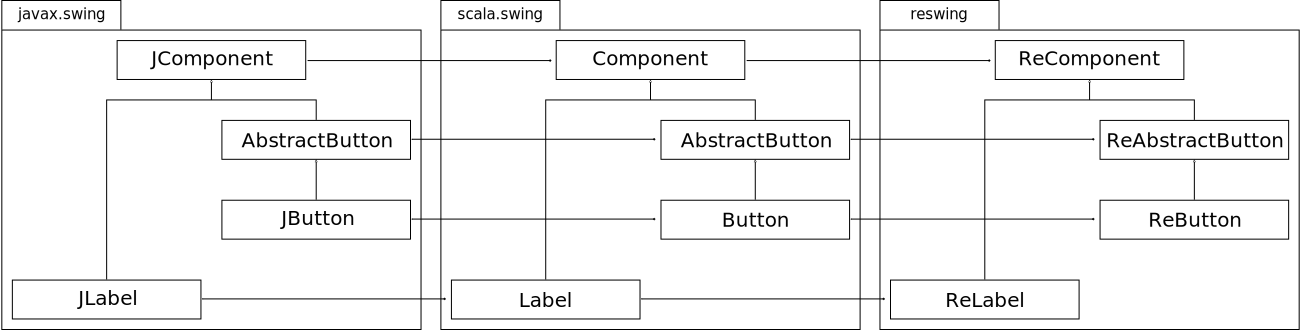
\includegraphics[width=0.5\textwidth]{images/overview}
  \caption{Scala Swing and ReSwing wrapper architecture}
  \label{fig:overview}
\end{figure}

The ReSwing library provides reactive values for properties of Swing
components. Since it is possible to define a signal for these values
and signals are defined once the signal is created and are not
re-assignable, properties in the ReSwing library are passed to the
components' constructors and cannot be assigned later {\bf Not
  clear}. This also results in a slightly different approach when
constructing ReSwing components as shown in
Figure~\ref{lst:scala-swing-example} and
Figure~\ref{lst:reswing-example}.


\begin{figure}[htp]
\begin{codenv}
val label = new Label
label.text = "foobar"
label.preferredSize = new Dimension(400, 40)
\end{codenv}
\caption{Label component instantiation in Scala Swing.}
\label{lst:scala-swing-example}
%\vspace{-4mm}
\end{figure}

\begin{figure}[htp]
\begin{codenv}
val label = new ReLabel(
    text = "foobar"
    preferredSize = new Dimension(400, 40)
)
\end{codenv}
\caption{ReLabel component instantiation in ReSwing.}
\label{lst:reswing-example}
%\vspace{-4mm}
\end{figure}


\subsection{ReSwing Events}
\label{sec:events}
The RESwing library provides REScala events for discrete changes,
e.g., button clicks. Events exposed by ReSwing components correspond
to Scala Swing events.  {\bf But more expressive power ? What about
  the parameter type ? What about combinators?}


\subsection{RESwing Reactive Values}
\label{sec:reactive-values}


RESwing bridges between the Scala Swing getter, setter and reactor
system and the REScala signal and event system. Clients can define
reactive values that are passed to the RESwing interface. When these
values change, the GUI interface is updated accordingly. Also, changes
made by the user are reflected in the reactive values which the
ReSwing library provides.

Certain values can be changed by both the application and the user,
i.e., they have multiple input sources. For example, the value
representing the text in a text input field is changed from the user
when she enters the text, ... {\bf What about the application?}. The
library ensures consistency between values set by the application and
those resulting from user interaction. This is achieved by disallowing
the user to make changes in certain cases.


There are three different ways to initialize a reactive value. This
aspect determines how changes to the reactive value are handled: {\bf
  show also the changes of the value}.

\begin{itemize}
\item \emph{Immediate value} will set the reactive value to the given
  value immediately upon creation. The user can change the value
  afterwards. {\bf How? Can you show it in the example?}
\item \emph{Event initialization} will update the reactive value on
  each event occurrence. The user can change the value by triggering
  an event in the stream with the new value.
\item \emph{Signal initialization} ensures that the reactive value
  always holds the value given by the signal. Hence, the user is not
  allowed to change the value after the initialization but the value
  automatically reflects the changes in the signal.
\end{itemize}

For all these cases, the respective value is passed to the constructor
of the component as shown in
Figure~\ref{lst:initializing-reactive-values}.

\begin{figure}[h]
\begin{codenv}
val value: String
val label = new ReTextArea(
    text = value 
)

val event: Event[String]
val label = new ReTextArea(
    text = event
)

val signal: Signal[String] 
val label = new ReTextArea( 
    text = signal 
)
\end{codenv}
\caption{Initializing a reactive value of a ReSwing component.}
\label{lst:initializing-reactive-values}
\end{figure}


After a component instance has been constructed, all reactive values
can be treated as signals when accessing the properties (e.g.,
\code{Signal \{ label.text() \}}). {\bf why not directly the signal? I
  would expect text is a signal}



\subsection{Extending the RESwing Library}
\label{sec:defining-reactive-values}
The library offers a declarative syntax to define which reactive value
should map to which property of the underlying Swing component. Using
this syntax ensures that value changes are properly propagated from
the ReSwing library to the Scala Swing library and vice versa.

For a reactive property, you need to specify:
\begin{itemize}
\item the \emph{getter} of the underlying Swing property to retrieve the value
\item the \emph{setter} of the underlying Swing property to set the
  value (if the reactive property can be changed by the application)
\item a way to identify changes of the underlying Swing property,
  either by giving the bound property name or a Scala Swing event type
\end{itemize}
Additionally it is possible to force other properties to hold a
specified value, if the reactive value should not be changeable by the
user. This can be the case if the reactive value is initialized with a
signal as described in \ref{sec:reactive-values}.

Examples of some reactive values defined in different ways are given
in \ref{lst:defining-reactive-values}.

\begin{figure}
\begin{codenv}
class ReLabel(val text: ReSwingValue[String] = ()) 
                             extends ReComponent {
  text using (peer.text _, peer.text_= _, "text")
}

class ReTextComponent(val text: ReSwingValue[String] = ()) 
                            extends ReComponent {
  (text using (peer.text _, peer.text_= _, classOf[ValueChanged])
        force ("editable", peer.editable_= _, false))
}

abstract class ReComponent extends ReUIElement {
  val hasFocus = ReSwingValue using (peer.hasFocus _, classOf[FocusGained],
                                                      classOf[FocusLost])
}
\end{codenv}
\caption{Defining Reactive Values.}
\label{lst:defining-reactive-values}
\vspace{-4mm}
\end{figure}



\end{document}
